\documentclass[12pt,fleqn]{article}
\setlength{\parindent}{0pt}
\usepackage{graphicx}
\usepackage{cancel}
\usepackage{listings}
\usepackage[latin5]{inputenc}
\usepackage{color}
\setlength{\parskip}{8pt}
\setlength{\parsep}{0pt}
\setlength{\headsep}{0pt}
\setlength{\topskip}{0pt}
\setlength{\topmargin}{0pt}
\setlength{\topsep}{0pt}
\setlength{\partopsep}{0pt}
\setlength{\mathindent}{0cm}
\usepackage{latexsym}
\usepackage{amsfonts}
\usepackage{showkeys}
\renewcommand*\showkeyslabelformat[1]{(#1)}

\begin{document}
Isi Denklemini Turetmek 

Bu denklemi turetmek icin ``enerjinini muhafazasi (conservation of
energy)'' kuralini kullanacagiz. Bu muhafaza kuralini bir esitlige
cevirecegiz, ve bu esitligi manipule ederek ortaya bir kismi turevsel
denklem (PDE) cikaratacagiz. Baz aldigimiz fiziksel ortam bir metal cubuk,
ki bu cubukta materyel yogunlugu her noktada ayni.  Formul soyle;

$[x,x+\Delta x]$ icindeki net isi degisim toplami = Tanimlanan bolge
sinirlarindaki isi akisi + $[x,x+\Delta x]$ icinde uretilen isi miktari

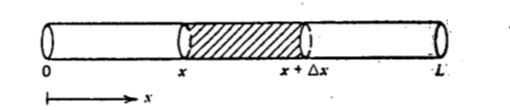
\includegraphics[height=2cm]{heat_1.png}

$[x,x+\Delta x]$ icindeki toplam isiyi nasil hesaplariz? Eger $u(x,t)$
metal cubugun $x$ noktasinda $t$ anindaki isiyi veriyorsa, verilen kesit
uzerinden bir entegral aliriz,

\[ [x,x+\Delta x] \textit{ Icindeki Toplam Isi} = 
cpA \int _{ x}^{x+\Delta x}u(s,t) ds
   \]



\[ \frac{d}{dt} \int _{ x}^{x+\Delta x} c\rho A u(s,t) ds = 
c\rho A  \frac{d}{dt} \int _{ x}^{x+\Delta x} u_t(s,t) ds
  \]


\[ = kA [ u_x(x+\Delta x,t) - u_x(x,t)] A \int _{x}^{x+\Delta x} f(s,t) ds \]

\[ \int _{ a}^{b} f(x) dx = f(\xi)(b-a)  \]

\[ c\rho A u_t(\xi_1,t)\Delta x = 
kA[u_x(x+\Delta x, t) - u_x(x,t)] + 
Af(\xi_2,t)\Delta x
 \]


\[ x < \xi < x+\Delta x \]

\[ u_t(\xi,t) = 
\frac{k}{c\rho} \bigg[
\frac{u_x(x+\Delta x,t) - u_x(x,t)}
{\Delta x}
\bigg]
+ \frac{ 1}{c\rho}f(\xi,t)
 \]

\[ \Delta x \to 0 \]

\[ u_t(x,t) = \alpha^2u_{xx}(x,t) + F(x,t) \]


Kaynaklar

Partial Differential Equations for Scientists and Engineers, Murlow, sf. 27

\end{document}
